\documentclass[portrait,final,a1paper,fontscale=0.401]{baposter}

\usepackage{calc}
\usepackage{graphicx}
\usepackage{amsmath}
\usepackage{amssymb}
\usepackage{relsize}
\usepackage{multirow}
\usepackage{rotating}
\usepackage{bm}
\usepackage{url}

\usepackage{setspace}

\usepackage{graphicx}
\usepackage{multicol}

%\usepackage{times}
%\usepackage{helvet}
%\usepackage{bookman}
\usepackage{palatino}

\newcommand{\captionfont}{\footnotesize}

\graphicspath{{images/}{../images/}}
\usetikzlibrary{calc}

\newcommand{\SET}[1]  {\ensuremath{\mathcal{#1}}}
\newcommand{\MAT}[1]  {\ensuremath{\boldsymbol{#1}}}
\newcommand{\VEC}[1]  {\ensuremath{\boldsymbol{#1}}}
\newcommand{\Video}{\SET{V}}
\newcommand{\video}{\VEC{f}}
\newcommand{\track}{x}
\newcommand{\Track}{\SET T}
\newcommand{\LMs}{\SET L}
\newcommand{\lm}{l}
\newcommand{\PosE}{\SET P}
\newcommand{\posE}{\VEC p}
\newcommand{\negE}{\VEC n}
\newcommand{\NegE}{\SET N}
\newcommand{\Occluded}{\SET O}
\newcommand{\occluded}{o}

%%%%%%%%%%%%%%%%%%%%%%%%%%%%%%%%%%%%%%%%%%%%%%%%%%%%%%%%%%%%%%%%%%%%%%%%%%%%%%%%
%%%% Some math symbols used in the text
%%%%%%%%%%%%%%%%%%%%%%%%%%%%%%%%%%%%%%%%%%%%%%%%%%%%%%%%%%%%%%%%%%%%%%%%%%%%%%%%

%%%%%%%%%%%%%%%%%%%%%%%%%%%%%%%%%%%%%%%%%%%%%%%%%%%%%%%%%%%%%%%%%%%%%%%%%%%%%%%%
% Multicol Settings
%%%%%%%%%%%%%%%%%%%%%%%%%%%%%%%%%%%%%%%%%%%%%%%%%%%%%%%%%%%%%%%%%%%%%%%%%%%%%%%%
\setlength{\columnsep}{1.5em}
\setlength{\columnseprule}{0mm}

%%%%%%%%%%%%%%%%%%%%%%%%%%%%%%%%%%%%%%%%%%%%%%%%%%%%%%%%%%%%%%%%%%%%%%%%%%%%%%%%
% Save space in lists. Use this after the opening of the list
%%%%%%%%%%%%%%%%%%%%%%%%%%%%%%%%%%%%%%%%%%%%%%%%%%%%%%%%%%%%%%%%%%%%%%%%%%%%%%%%
\newcommand{\compresslist}{%
\setlength{\itemsep}{1pt}%
\setlength{\parskip}{0pt}%
\setlength{\parsep}{0pt}%
}

%%%%%%%%%%%%%%%%%%%%%%%%%%%%%%%%%%%%%%%%%%%%%%%%%%%%%%%%%%%%%%%%%%%%%%%%%%%%%%
%%% Begin of Document
%%%%%%%%%%%%%%%%%%%%%%%%%%%%%%%%%%%%%%%%%%%%%%%%%%%%%%%%%%%%%%%%%%%%%%%%%%%%%%

\begin{document}

%%%%%%%%%%%%%%%%%%%%%%%%%%%%%%%%%%%%%%%%%%%%%%%%%%%%%%%%%%%%%%%%%%%%%%%%%%%%%%
%%% Here starts the poster
%%%---------------------------------------------------------------------------
%%% Format it to your taste with the options
%%%%%%%%%%%%%%%%%%%%%%%%%%%%%%%%%%%%%%%%%%%%%%%%%%%%%%%%%%%%%%%%%%%%%%%%%%%%%%
% Define some colors

%\definecolor{lightblue}{cmyk}{0.83,0.24,0,0.12}
\definecolor{lightblue}{rgb}{0.5,0.8,1}
\definecolor{darkblue}{rgb}{0.5,0.8,1}
\definecolor{myblue}{rgb}{0.2,0.7,0.2}

% Draw a video
\newlength{\FSZ}
\newcommand{\drawvideo}[3]{% [0 0.25 0.5 0.75 1 1.25 1.5]
   \noindent\pgfmathsetlength{\FSZ}{\linewidth/#2}
   \begin{tikzpicture}[outer sep=0pt,inner sep=0pt,x=\FSZ,y=\FSZ]
   \draw[color=lightblue!50!black] (0,0) node[outer sep=0pt,inner sep=0pt,text width=\linewidth,minimum height=0] (video) {\noindent#3};
   \path [fill=lightblue!50!black,line width=0pt] 
     (video.north west) rectangle ([yshift=\FSZ] video.north east) 
    \foreach \x in {1,2,...,#2} {
      {[rounded corners=0.6] ($(video.north west)+(-0.7,0.8)+(\x,0)$) rectangle +(0.4,-0.6)}
    }
;
   \path [fill=lightblue!50!black,line width=0pt] 
     ([yshift=-1\FSZ] video.south west) rectangle (video.south east) 
    \foreach \x in {1,2,...,#2} {
      {[rounded corners=0.6] ($(video.south west)+(-0.7,-0.2)+(\x,0)$) rectangle +(0.4,-0.6)}
    }
;
   \foreach \x in {1,...,#1} {
     \draw[color=lightblue!50!black] ([xshift=\x\linewidth/#1] video.north west) -- ([xshift=\x\linewidth/#1] video.south west);
   }
   \foreach \x in {0,#1} {
     \draw[color=lightblue!50!black] ([xshift=\x\linewidth/#1,yshift=1\FSZ] video.north west) -- ([xshift=\x\linewidth/#1,yshift=-1\FSZ] video.south west);
   }
   \end{tikzpicture}
}

\hyphenation{resolution occlusions}
%%
\begin{poster}%
  % Poster Options
  {
  % Show grid to help with alignment
  grid=false,
  % Column spacing
  colspacing=1em,
  % Color style
  bgColorOne=white,
  bgColorTwo=white,
  borderColor=lightblue,
  headerColorOne=darkblue,
  headerColorTwo=lightblue,
  headerFontColor=black,
  boxColorOne=white,
  boxColorTwo=lightblue,
  % Format of textbox
  textborder=roundedleft,
  % Format of text header
  eyecatcher=true,
  headerborder=closed,
  headerheight=0.1\textheight,
%  textfont=\sc, An example of changing the text font
  headershape=roundedright,
  headershade=shadelr,
  headerfont=\Large\bf\textsc, %Sans Serif
  textfont={\setlength{\parindent}{0.5em}},
  boxshade=plain,
%  background=shade-tb,
  background=plain,
  linewidth=2pt
  }
  % Eye Catcher
  {} 
  % Title
  {\bf\textsc{Additive regularization of topic models: \\ Convergence results}\vspace{0.5em}}
  % Authors
  {\textsc{Ilya Irkhin, ilirhin@gmail.com }}
  % University logo
  {% The makebox allows the title to flow into the logo, this is a hack because of the L shaped logo.
    %\includegraphics[height=9.0em]{images/msu.png}
  }

%%%%%%%%%%%%%%%%%%%%%%%%%%%%%%%%%%%%%%%%%%%%%%%%%%%%%%%%%%%%%%%%%%%%%%%%%%%%%%
%%% Now define the boxes that make up the poster
%%%---------------------------------------------------------------------------
%%% Each box has a name and can be placed absolutely or relatively.
%%% The only inconvenience is that you can only specify a relative position 
%%% towards an already declared box. So if you have a box attached to the 
%%% bottom, one to the top and a third one which should be in between, you 
%%% have to specify the top and bottom boxes before you specify the middle 
%%% box.
%%%%%%%%%%%%%%%%%%%%%%%%%%%%%%%%%%%%%%%%%%%%%%%%%%%%%%%%%%%%%%%%%%%%%%%%%%%%%%
    

%%%%%%%%%%%%%%%%%%%%%%%%%%%%%%%%%%%%%%%%%%%%%%%%%%%%%%%%%%%%%%%%%%%%%%%%%%%%%%
\headerbox{Problem statement}{name=statement, column=0, row=0, span=3}{
ARTM combines regularizers to let user build topic models with a rich set of desired properties. 
\medskip

\textbf{Problem}: find convergence test for regularized EM-algorithm; propose modifications of the algorithm to ensure convergence of the algorithm.
}

%%%%%%%%%%%%%%%%%%%%%%%%%%%%%%%%%%%%%%%%%%%%%%%%%%%%%%%%%%%%%%%%%%%%%%%%%%%%%%
\headerbox{Topic modeling}{name=topicmodeling,column=0, below=statement}{
%%%%%%%%%%%%%%%%%%%%%%%%%%%%%%%%%%%%%%%%%%%%%%%%%%%%%%%%%%%%%%%%%%%%%%%%%%%%%%
	\textbf{Given:}
	
	$ D $ is a set of documents, $ W $ is a set of terms, $n_{dw}$ is a frequency of term $w$ in document $d$.
	
	\medskip\textbf{Find} model: 
	\[ 
	p(w|d) = \sum_{t\in T} p(w|t) p(t|d) = \sum_{t\in T} \varphi_{wt} \theta_{td}
	\] 
	with parameters $\varphi_{wt}$, $\theta_{td}$:
	\begin{itemize}
	\item $ \varphi_{wt} = p(w|t)$ is a distribution over terms in topic $ t $;
	\item $ \theta_{td} = p(t|d) $ is a distribution over topics in document $ d $. 
	\end{itemize}
	
	\textbf{Optimization task} is
	regularized likelihood maximization:
  \[\small
        \underbrace{\sum_{d\in D} \sum_{w\in d} \!n_{dw} \ln \sum_{t\in T} \phi_{wt}\theta_{td}}_{L(\Phi,\Theta)}
        +
        {\underbrace{{\sum_{i=1}^n \tau_i R_i(\Phi,\Theta)}}_{R(\Phi,\Theta)}}
        \to \max _{\Phi,\Theta}
   \]
	 where $R(\Phi, \Theta)$ is a weighted sum of regularization criteria.
	  \vspace{2.4em}
  }
  
%%%%%%%%%%%%%%%%%%%%%%%%%%%%%%%%%%%%%%%%%%%%%%%%%%%%%%%%%%%%%%%%%%%%%%%%%%%%%%
  
\headerbox{Convergence theorem}{name=convergence,column=1,below=statement}{
Let $k$ be the the index of the iteration. Suppose the following conditions are satisfied:
\begin{enumerate}
\item  Preserving zeros.
\smallskip

$ n^k_{wt} = 0 \Rightarrow \phi^k_{wt} = 0$ , $n^k_{td} = 0 \Rightarrow \theta^k_{td} = 0$.
\item Separation from zero of $\phi$ and $\theta$.
\smallskip

$\exists \varepsilon>0\ \exists N\ \forall k > N\ \phi^k_{wt}, \theta^k_{td} \notin (0, \varepsilon)$. 
\item  Likelihood is finite during iterations.
\smallskip

$ n_{dw}>0 \Rightarrow \forall k\ \exists t\colon p^k_{tdw} > 0$.
\item Separation of the denominator.
\smallskip

$\exists \delta >0\ \exists N\ \forall k > N \ \forall t\ \exists w\  n^k_{wt} + r^k_{wt} > \delta$ and the similar condition for $\theta$. 
\item Growth of the lower bound of regularized likelihood during iterations.
\smallskip

$\exists N\ \forall k > N\colon\ \ Q^k (\phi^k, \theta^k)+ R(\phi^k, \theta^k) \geq Q^k(\phi^{k-1}, \theta^{k-1}) + R(\phi^{k-1}, \theta^{k-1})$, where $Q^k(\phi, \theta) = \sum\limits_{t,d,w} p^k_{tdw} (\ln \phi_{wt} + \ln \theta_{td})$.
\end{enumerate}
Then for  $k \to \infty$
\smallskip

$\|\phi^k - \phi^{k-1}\|_1 \to 0 \text{ and }\|\theta^k - \theta^{k-1}\|_1 \to 0$ .
}


%%%%%%%%%%%%%%%%%%%%%%%%%%%%%%%%%%%%%%%%%%%%%%%%%%%%%%%%%%%%%%%%%%%%%%%%%%%%%%
\headerbox{Regularized EM}{name=regem, column=2, below=statement}{
    Karush-Kuhn-Tucker theorem justifies the following EM-algorithm:
    
   \textbf{E-step:}
    
    $p_{tdw} \propto \varphi_{wt} \theta_{td}$
 \smallskip
   
    \textbf{M-step:}
    
    $n_{wt} = \sum\limits_{d \in D} n_{dw} p_{tdw}$
    
    $n_{td} = \sum\limits_{w \in W} n_{dw} p_{tdw}$
    
   $r_{wt} =  \phi_{wt}\tfrac{\partial R}{\partial\phi_{wt}}$,~~ $r_{td} =  \theta_{td}\tfrac{\partial R}{\partial\theta_{td}}$

    $\phi_{wt}   \propto \bigl(n_{wt} + r_{wt} \bigr)_{\!+}$,~~ $\theta_{td} \propto  \bigl(n_{td} + r_{td}\bigr)_{\!+}$
}


%%%%%%%%%%%%%%%%%%%%%%%%%%%%%%%%%%%%%%%%%%%%%%%%%%%%%%%%%%%%%%%%%%%%%%%%%%%%%%
\headerbox{Unbiased Modification}{name=unbiasedem,column=2,below=regem}{
    Replacing $\phi_{wt}$ and $\theta_{td}$ with their unbiased maximum likelihood estimators on M-step preserves the convergence and simplifies calculations:
 \smallskip
    
  $ r_{wt} =  \dfrac{n_{wt}}{n_t}\dfrac{\partial R}{\partial\phi_{wt}} \bigg( \dfrac{n_{wt}}{n_t},  \dfrac{n_{td}}{n_d} \bigg)$
 \smallskip
 
   $r_{td} =\dfrac{n_{td}}{n_d}\dfrac{\partial R}{\partial\theta_{td}}  \bigg( \dfrac{n_{wt}}{n_t},  \dfrac{n_{td}}{n_d} \bigg)$
 \smallskip
 
    Under conditions of the convergence theorem and with this modification  one can estimate the change of $R$ on M-step:
\[
\Delta R=  \frac12 \sum\limits_{t, w, u}   \frac{1}{\sum\limits_v n_{vt}} \bigg(  \frac{\partial{R}}{\partial{\phi_{wt}}}  -  \frac{\partial{R}}{\partial{\phi_{ut}}}  \bigg)^2 \phi_{wt} \phi_{ut}  + 
\]
\[
+ \frac12 \sum\limits_{d, t, s}   \frac{1}{\sum\limits_r n_{rd}} \bigg(  \frac{\partial{R}}{\partial{\theta_{td}}}  -  \frac{\partial{R}}{\partial{\theta_{sd}}}  \bigg)^2 \theta_{td} \theta_{sd}  \geq 0
\]
}


%%%%%%%%%%%%%%%%%%%%%%%%%%%%%%%%%%%%%%%%%%%%%%%%%%%%%%%%%%%%%%%%%%%%%%%%%%%%%%

\headerbox{Gradient Modification}{name=gradientem,column=2,below=unbiasedem}{
Using the gradient of regularizer as $r_{wt}$ and $r_{td}$ may improve the convergence and does not complicate the calculations.
\smallskip
\smallskip

$r_{wt} =  \frac{1}{\sum\limits_w n_{wt}} \big( \frac{\partial{R}}{\partial{\phi_{wt}}} - \sum\limits_u \phi_{ut} \frac{\partial{R}}{\partial{\phi_{ut}}} \big)$

$ r_{td} =  \frac{1}{\sum\limits_t n_{td}} \big( \frac{\partial{R}}{\partial{\theta_{td}}} - \sum\limits_s \theta_{sd} \frac{\partial{R}}{\partial{\theta_{sd}}} \big)$
\smallskip

The negative additive is common for all topics (documents) so it can be efficiently computed without impacting the asymptotic of the algorithm.
}

%%%%%%%%%%%%%%%%%%%%%%%%%%%%%%%%%%%%%%%%%%%%%%%%%%%%%%%%%%%%%%%%%%%%%%%%%%%%%%

\headerbox{Conclusion}{name=conclusion,column=2,below=gradientem}{
1. We obtained simple conditions for the weak convergence of EM-algorithm.

2.  We proposed two modifications of M-step: unbiased and gradient, which improve the convergence without increasing the computaional complexity.
}

%%%%%%%%%%%%%%%%%%%%%%%%%%%%%%%%%%%%%%%%%%%%%%%%%%%%%%%%%%%%%%%%%%%%%%%%%%%%%%
 
  
\headerbox{Experiments}{name=experiment,column=0,below=convergence, span=2}{ 
We use dataset obtained from sport news website, $|D|=18000$, $|W|=20000$, $|T|=7$. We compare three variations of M-step (original, unbiased modification and gradient modification).  EM algorithm was launched from 200 random initial states and functionals were averaged over iterations. Results are presented below for decorrelation regularizer ($R = \tau\sum_{t, w\neq u} \phi_{wt}\phi_{ut}$)  with different values of $\tau$ ($-10^5, -10^6$).
 }



%%%%%%%%%%%%%%%%%%%%%%%%%%%%%%%%%%%%%%%%%%%%%%%%%%%%%%%%%%%%%%%%%%%%%%%%%%%%%%
\headerbox{Optimization trajectory}{name=pictures, column=0, below=experiment, span=2}{
\center{ 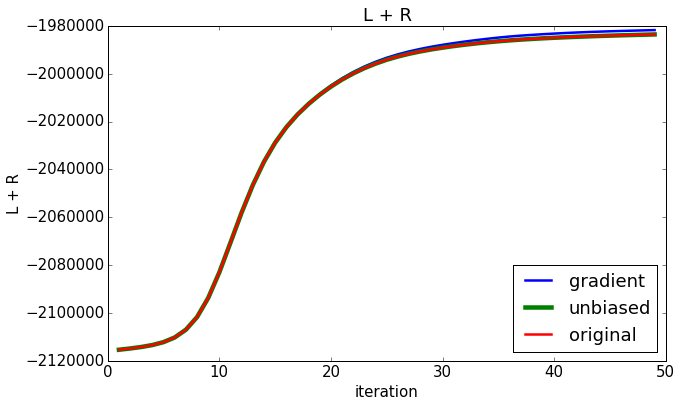
\includegraphics[width=0.43\linewidth]{LR5}
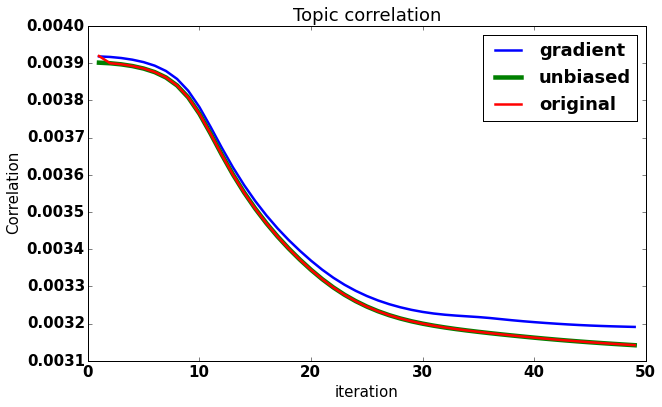
\includegraphics[width=0.43\linewidth]{R5}}\\
\center{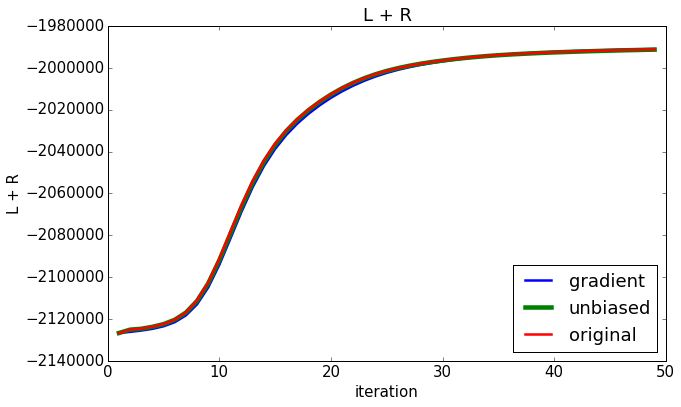
\includegraphics[width=0.43\linewidth]{LR6}
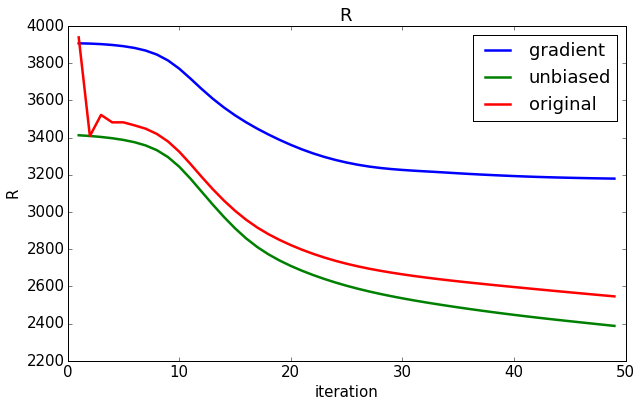
\includegraphics[width=0.43\linewidth]{R6}}\\
}

%%%%%%%%%%%%%%%%%%%%%%%%%%%%%%%%%%%%%%%%%%%%%%%%%%%%%%%%%%%%%%%%%%%%%%%%%%%%%%

\headerbox{References}{name=references,column=0,below=pictures,span=3}{
\textit{Vorontsov K. V., Potapenko A. A.} Additive Regularization of Topic Models // Machine Learning. Special Issue ''Data Analysis and Intelligent Optimization with Applications'': Volume 101, Issue 1 (2015), Pp. 303-323.
}

\end{poster}
\end{document}

